%%%%%%%%%%%%%%%%%%%%%%%%%%%%%%%%%%%%%%%%%
% a0poster Portrait Poster
% LaTeX Template
% Version 1.0 (22/06/13)
%
% The a0poster class was created by:
% Gerlinde Kettl and Matthias Weiser (tex@kettl.de)
% 
% This template has been downloaded from:
% http://www.LaTeXTemplates.com
%
% License:
% CC BY-NC-SA 3.0 (http://creativecommons.org/licenses/by-nc-sa/3.0/)
%
%%%%%%%%%%%%%%%%%%%%%%%%%%%%%%%%%%%%%%%%%

%----------------------------------------------------------------------------------------
%	PACKAGES AND OTHER DOCUMENT CONFIGURATIONS
%----------------------------------------------------------------------------------------

\documentclass[a0, landscape]{a0poster}
\usepackage{multicol} % This is so we can have multiple columns of text side-by-side
\columnsep=100pt 
\columnseprule = 3pt% This is the amount of white space between the columns in the poster
 % This is the thickness of the black line between the columns in the poster

\usepackage[svgnames]{xcolor} % Specify colors by their 'svgnames', for a full list of all colors available see here: http://www.latextemplates.com/svgnames-colors

\usepackage{times} % Use the times font
%\usepackage{palatino} % Uncomment to use the Palatino font

\usepackage{graphicx} % Required for including images
\graphicspath{{figures/}}
\usepackage{booktabs} % Top and bottom rules for table
\usepackage[font=small,labelfont=bf, skip=0pt]{caption} % Required for specifying captions to tables and figures
\usepackage{amsfonts, amsmath, amsthm, amssymb} % For math fonts, symbols and environments
\usepackage{wrapfig} % Allows wrapping text around tables and figures
\usepackage{titlesec}
\let\oldenumerate\enumerate
\renewcommand{\enumerate}{
	\oldenumerate
	\setlength{\itemsep}{0pt}
	\setlength{\parskip}{0pt}
	\setlength{\parsep}{0pt}
}

\let\olditemize\itemize
\renewcommand{\itemize}{
	\olditemize
	\setlength{\itemsep}{0pt}
	\setlength{\parskip}{0pt}
	\setlength{\parsep}{0pt}
}

\setlength{\parindent}{0pt}
\titlespacing*{\section}{0pt}{10pt}{10pt}

\usepackage{lmodern}
\usepackage[firstinits=true,backend=bibtex,doi=false,isbn=false,url=true]{biblatex}
\AtEveryBibitem{%
	\clearfield{pages}%
}
\renewcommand{\bibfont}{\normalfont\footnotesize}
\addbibresource{references.bib}

\defbibenvironment{bibliography}
{\noindent}
{\unspace}
{\printtext[bold]{\printtext[labelnumberwidth]{%
			\printfield{prefixnumber}%
			\printfield{labelnumber}}}
	\addspace}
\renewbibmacro*{finentry}{\finentry\quad}

\begin{document}

%----------------------------------------------------------------------------------------
%	POSTER HEADER 
%----------------------------------------------------------------------------------------



\begin{minipage}[b]{1\linewidth}
\Huge \textbf{An Online Algorithm For A Low Cost Real-Time Sensor-Based Fenceline Leak Detection System} \color{Black}\\ % Title
\Large \textbf{Halley Brantley, Yichen Si, \& Dendi Suhubdy}\\[0.5cm] % Author(s)
\large  North Carolina State University \\[0.4cm] % University/organization
\end{minipage}

\vspace{-20mm}

\begin{multicols}{3} % This is how many columns your poster will be broken into, a portrait poster is generally split into 2 columns


%----------------------------------------------------------------------------------------
%	INTRODUCTION
%----------------------------------------------------------------------------------------


\section*{Introduction}
Benzene is an air pollutant and carcinogen that is regulated by the U.S. Environmental Protection Agency (EPA) and often emitted by petroleum refineries as a result of leaking equipment and wastewater treatment \cite{fencelinerule}. Cost-effective and real-time methods for monitoring hazardous air pollutants emitted from industrial facilities could lead to faster leak detection, repair, and reduced emissions. One monitoring method currently under development by the EPA's Office of Research and Development is the SEnsor NeTwork INtelligent Emission Locator (SENTINEL) that combines time-resolved measurements and inverse models of various forms to improve source understanding on a variety of spatial scales. We present here an algorithm for locating the source of emissions using 1-sec benzene sensor and wind data.  
\vspace{10pt}

\section*{Data Description}
\begin{minipage}{.14\textwidth}
	\begin{center}
		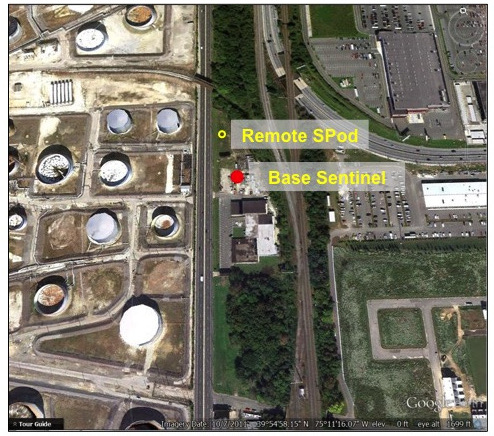
\includegraphics[width=\linewidth]{Slide11}
	\end{center}
\end{minipage}%
\hfill
\begin{minipage}{.14\textwidth}
	\begin{center}	
		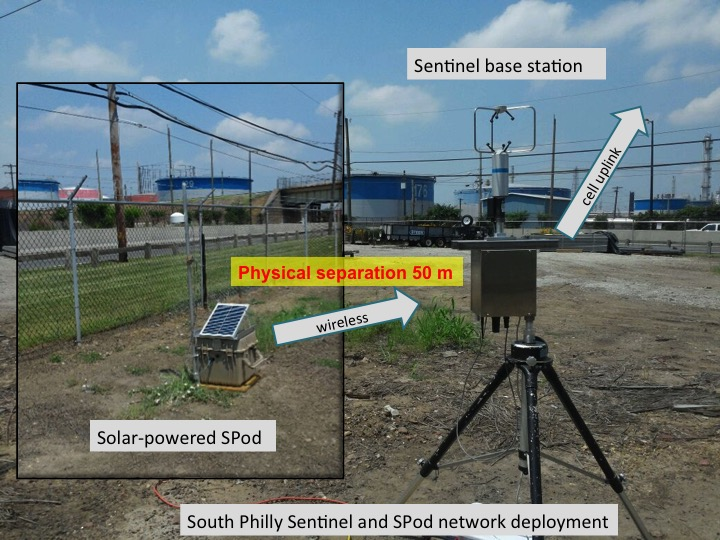
\includegraphics[width=\linewidth]{Slide12}			
	\end{center}
\end{minipage}
\vspace{40pt}
\begin{itemize}
		\item Solar-powered "sensor pod" (SPod) controlled by a low cost and low power Arduino UNO computer
		\item Wired SENTINEL base station containing an Intel Atom\textsuperscript{TM} computer (Santa Clara, CA, USA) and a model 81000V 3-D Ultrasonic Anemometer (R.M. Young, Inc., Traverse City, MI, USA) for 1 Hz wind measurements.
		\item Both systems log time-synchronized 1 Hz data from a custom EPA-developed sensor board containing a 10.6 eV passive photoionization detector [PID] (blue label piD-TECH \textsuperscript{\textregistered}, Baseline-Mocon Inc. Lyons, CO, USA) used to detect VOCs (benzene). 
		\item Deployed near a refinery in South Philadelphia from July, 2014 through February, 2015. Data from November, 2014 is analyzed here as an illustration.
		\item PID sensor response and stability are affected by temperature, humidity, lamp deposition and other variables resulting in unwanted baseline drift that complicates data analysis.	
		\item The PID sensor output ranges from 0.2 to 5 volts. 	
\end{itemize} 
\vspace{20pt}
\begin{center}
	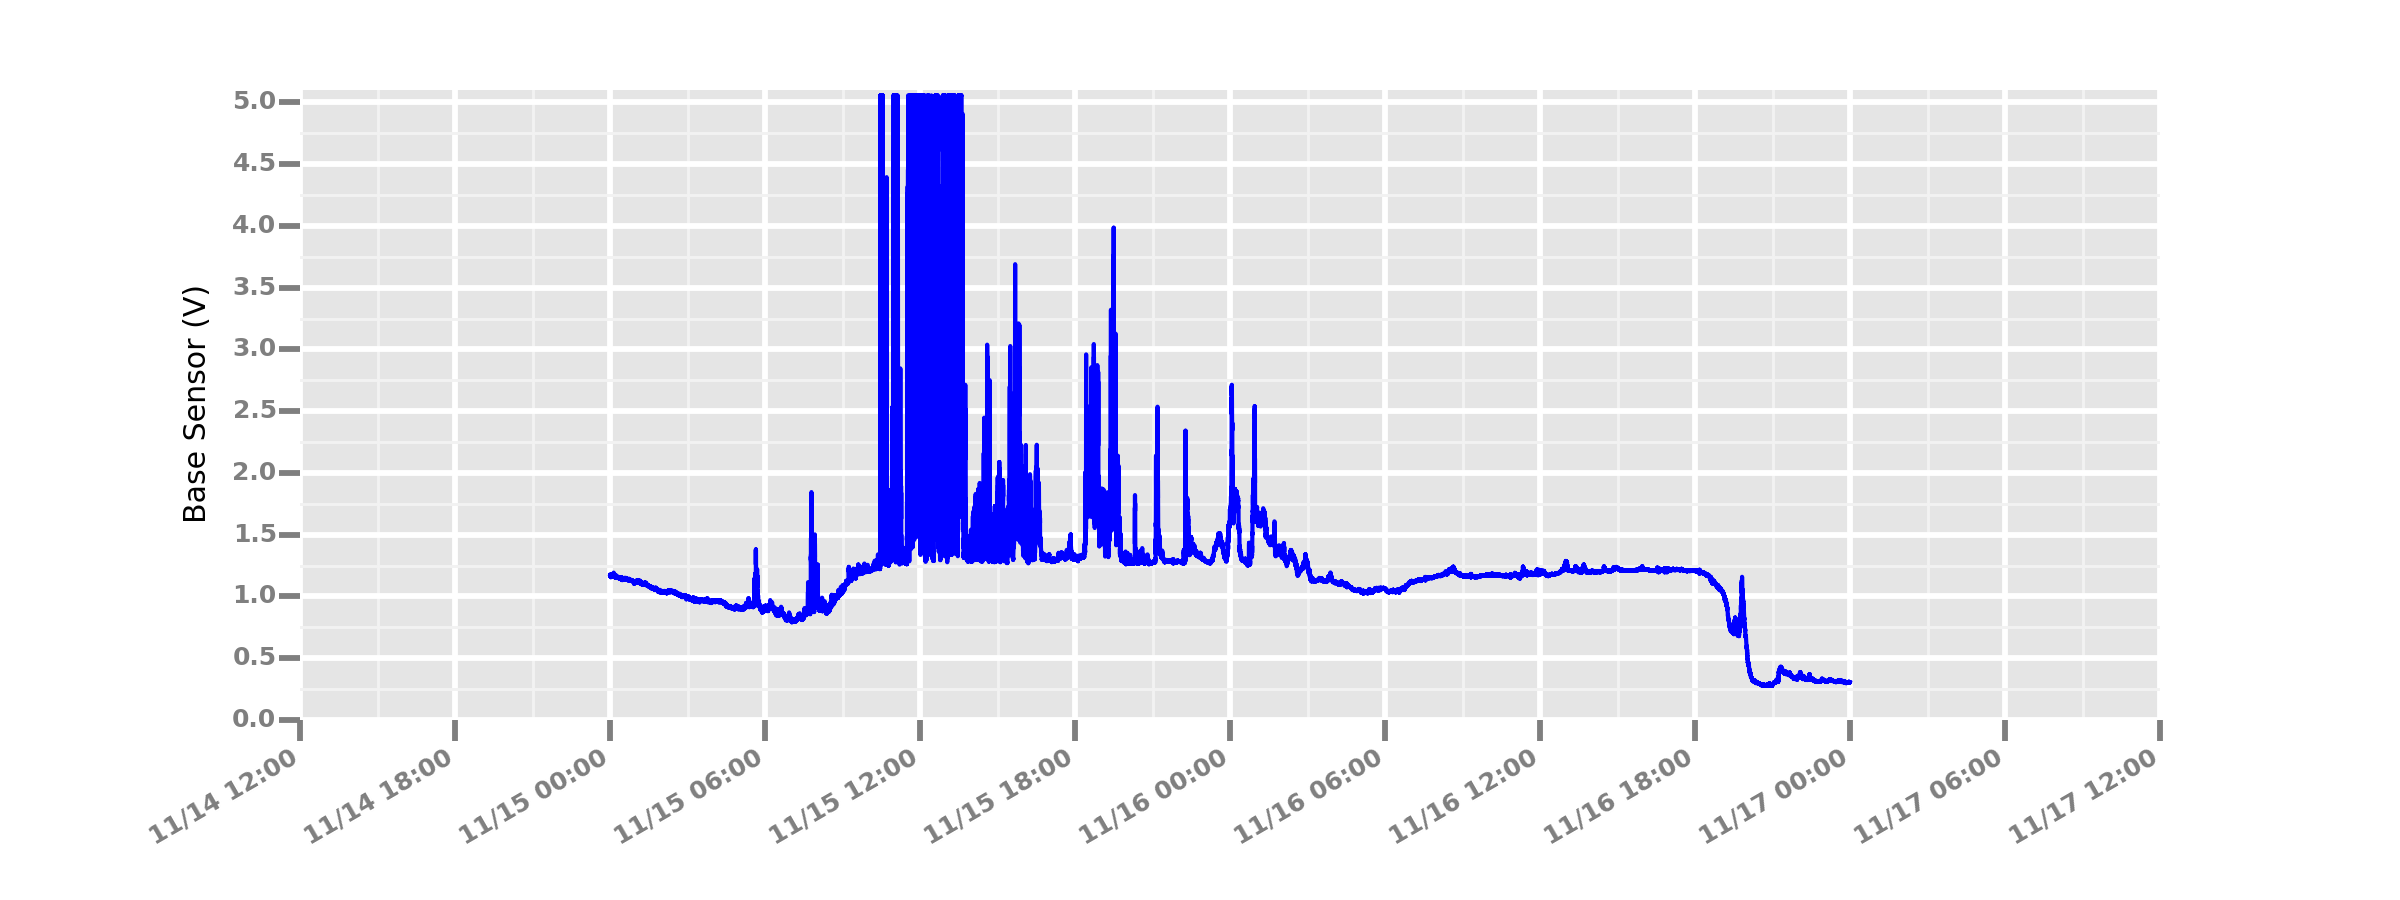
\includegraphics[width=\linewidth]{Base}
	\captionof{figure}{Example Base Sensor Signal}
	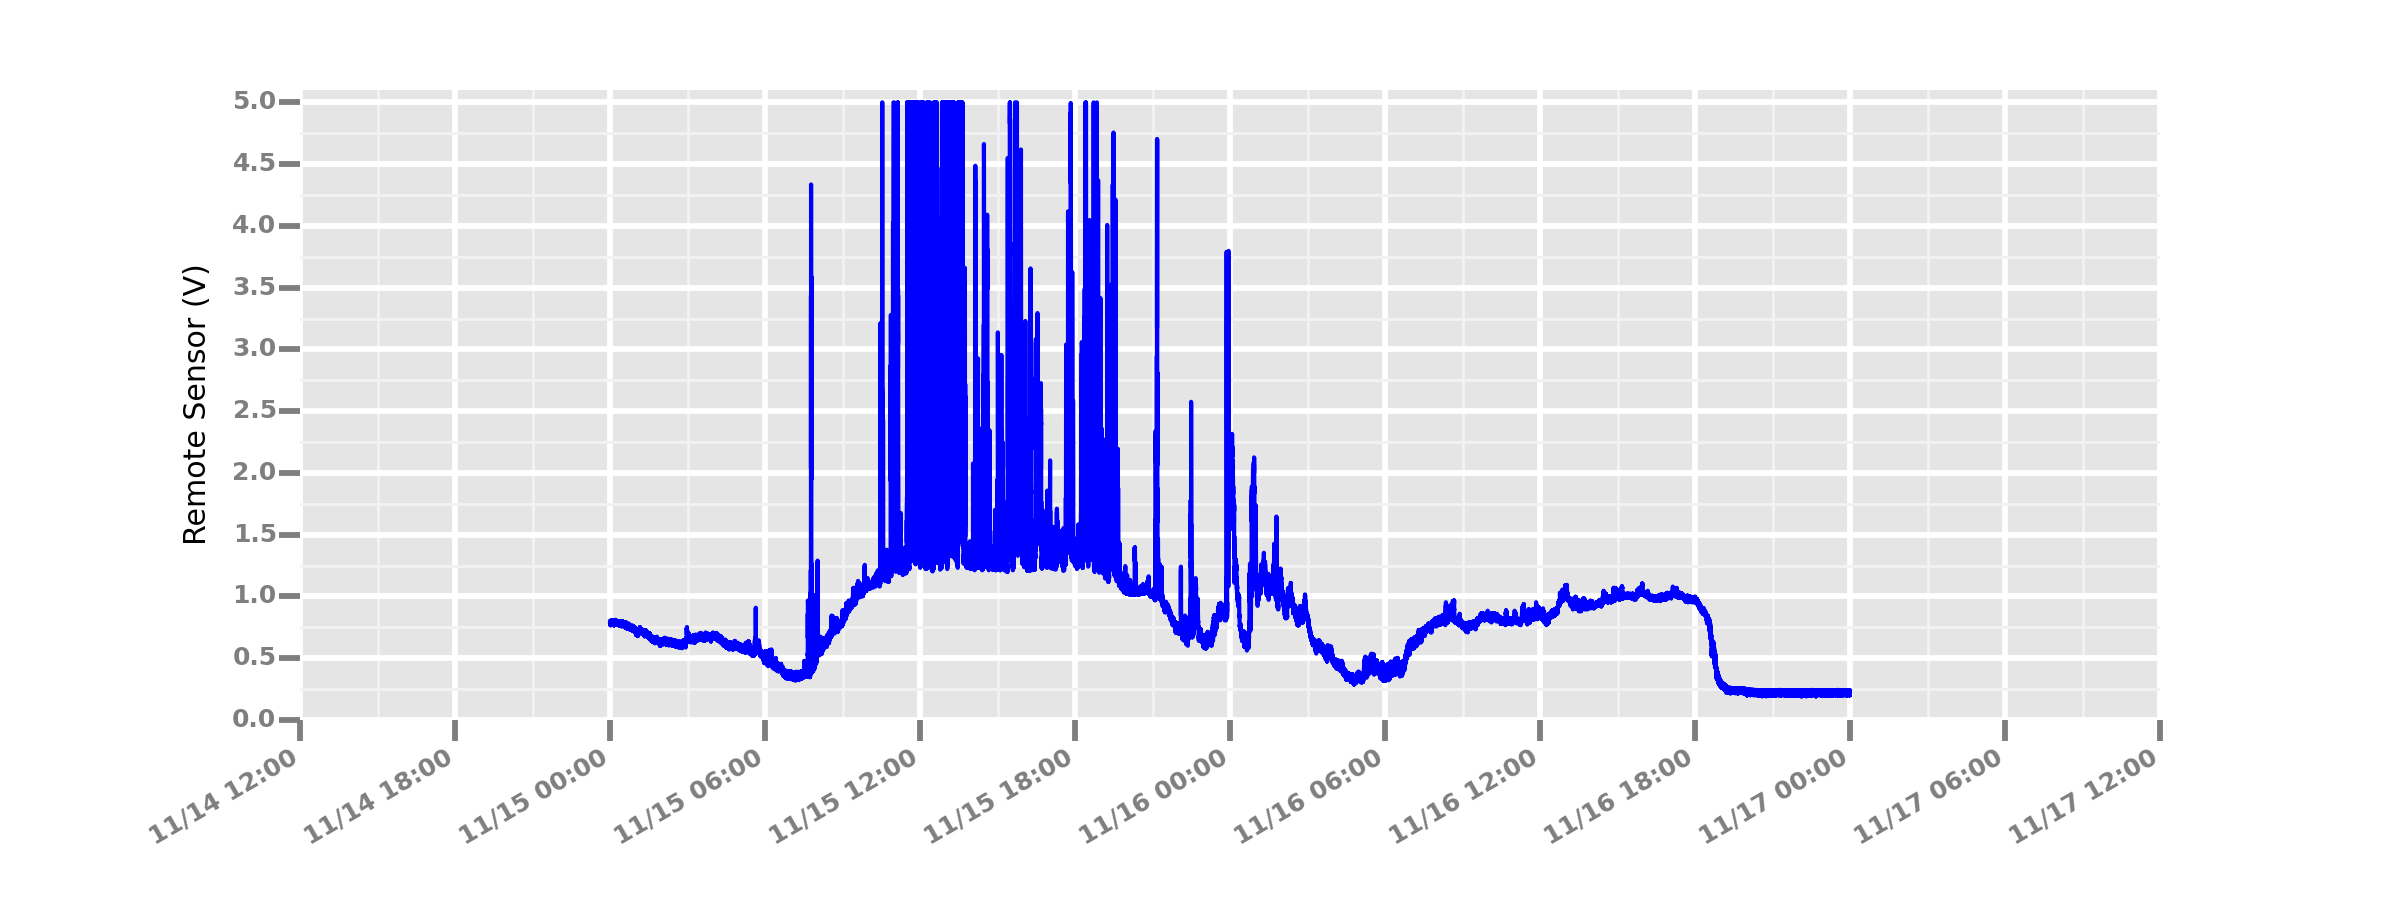
\includegraphics[width=\linewidth]{Remote}
	\captionof{figure}{Example SPod Sensor Signal}	
\end{center}

\section*{Simulated Data}
\begin{minipage}{.14\textwidth}
\begin{itemize}
	\item Time series for one day were simulated for each of the sensors.  
	\item Concentration was simulated at 0.05 Hz using the QUIC Dispersion Modeling System \cite{QUIC} and 5 min averaged wind measurements and up-sampled to 1 Hz by repeating the previous value. 
	\item Each hour of the stochastic baseline was simulated as 1D Brownian bridge with each step drawn from a standard normal.
	\item An offset of 1.5 was added to the simulated baseline, to imitate the measured values
	\item After the simulated baseline and concentration were added, values above above 5 were censored to 5 and values below 0.25 were replace with random draws from a $N(0.25, 0.05)$ 
\end{itemize}
\end{minipage}
\hfill
\begin{minipage}{.15\textwidth}
	\begin{center}			
		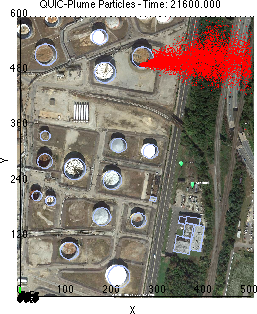
\includegraphics[width=\linewidth]{QUIC_fig}
		\captionof{figure}{QUIC Plume Visualization}	
	\end{center}
\end{minipage}

\begin{center}			
	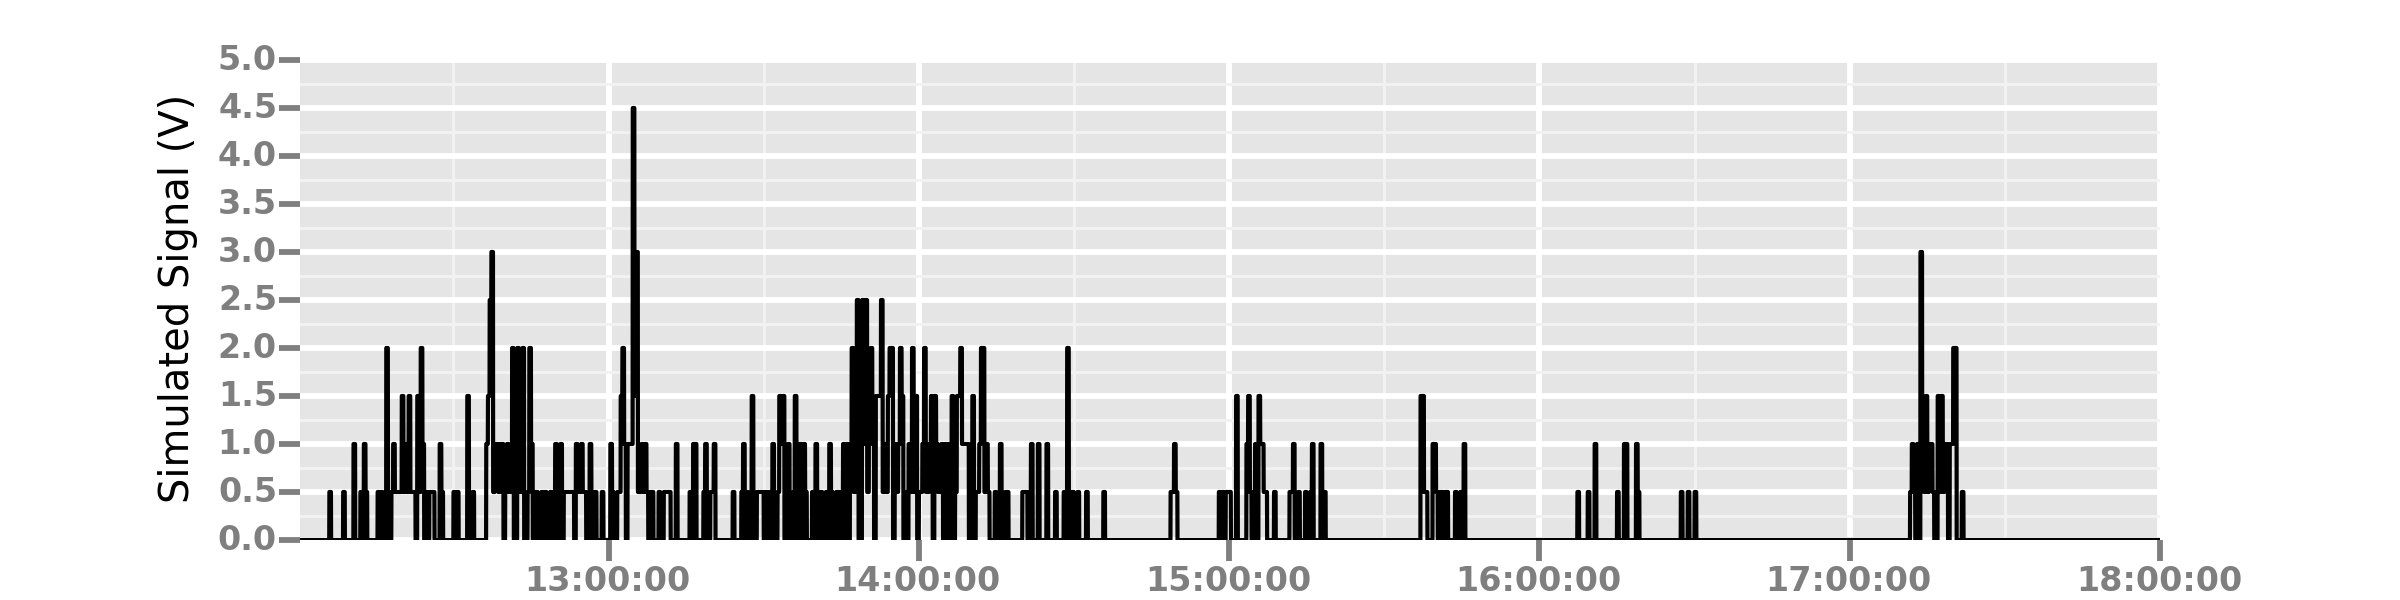
\includegraphics[width=\linewidth]{BaseSim}
	\captionof{figure}{Base Sensor Simulated Concentration from QUIC}
	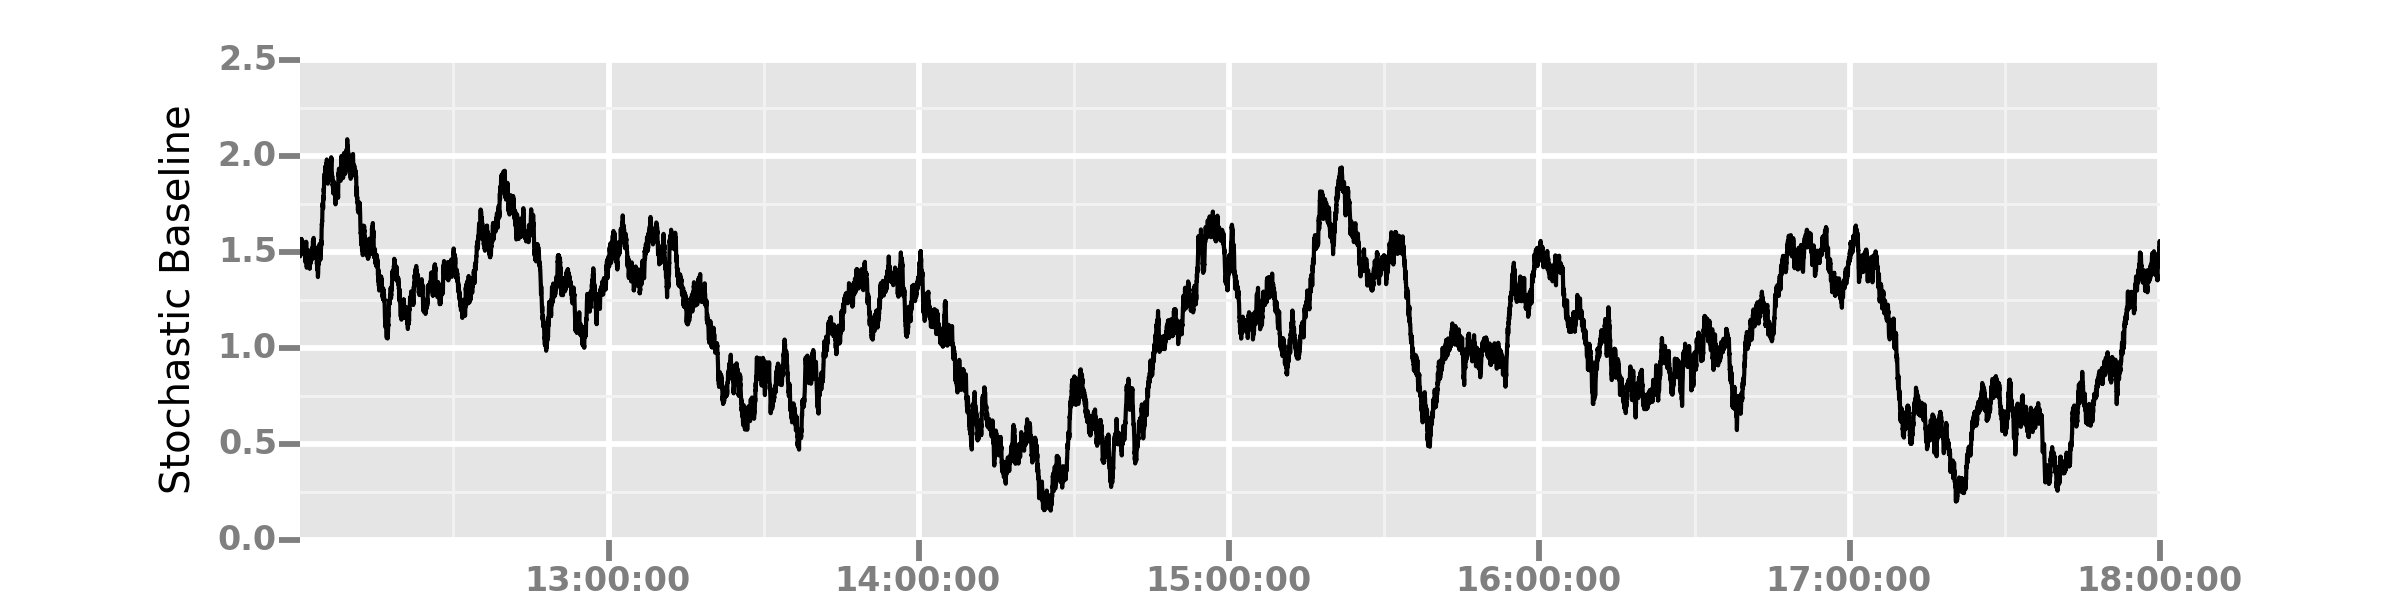
\includegraphics[width=\linewidth]{BaseRand}
	\captionof{figure}{Base Sensor Simulated Stochastic Baseline}
	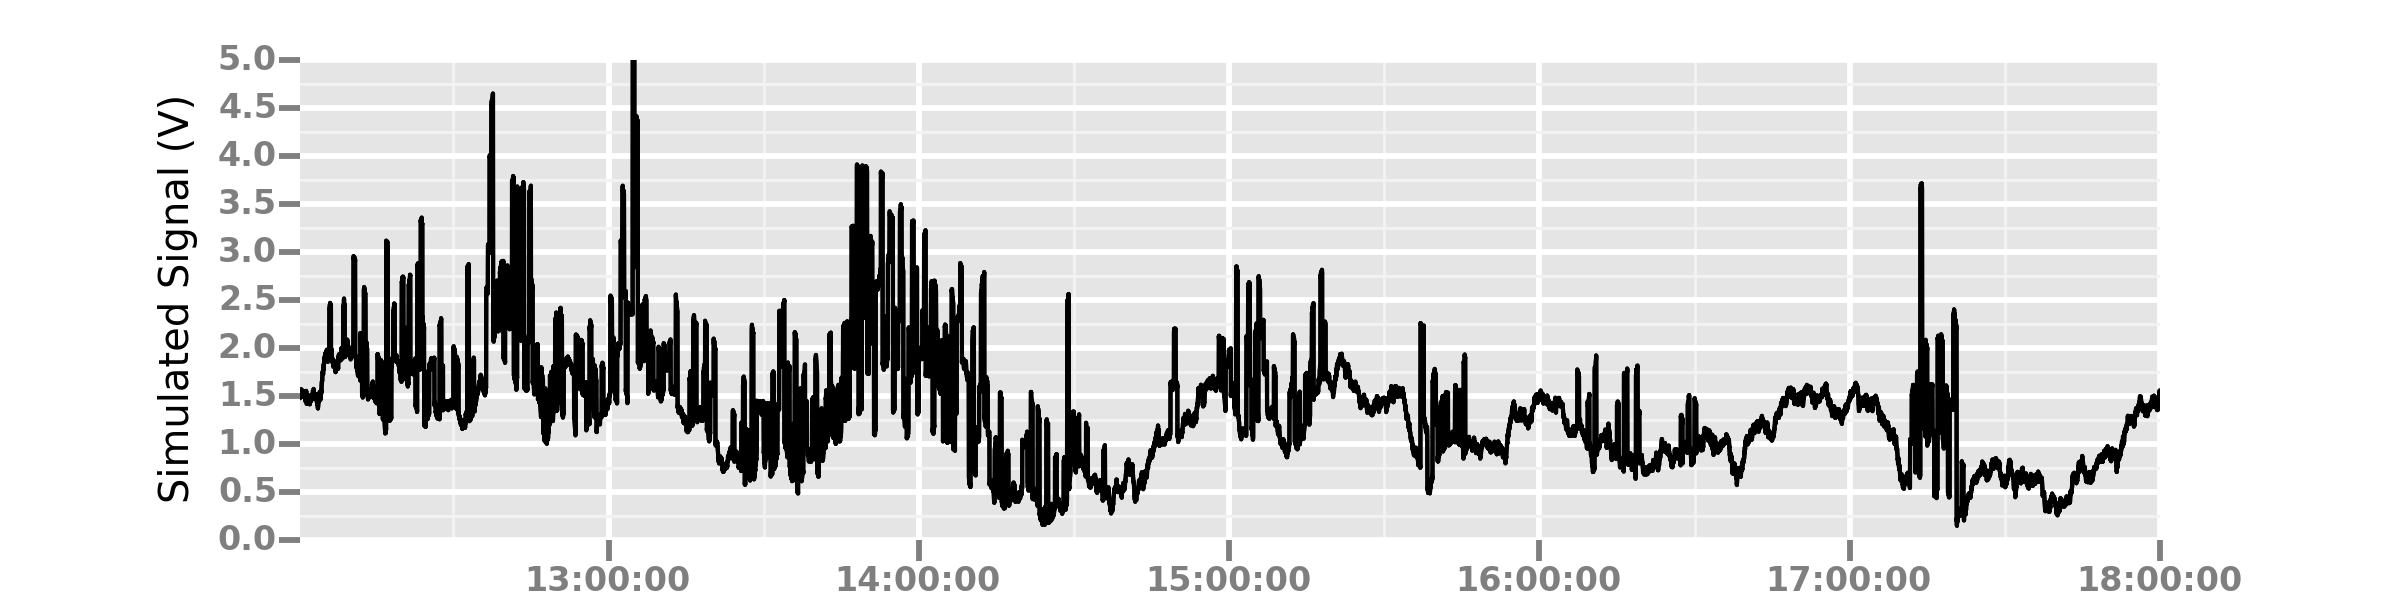
\includegraphics[width=\linewidth]{BaseTotal}
	\captionof{figure}{Base Sensor Simulated Data}
	\includegraphics[width=\linewidth]{RemoteTotal}
	\captionof{figure}{SPod Sensor Simulated Data}	
\end{center}


%------------------------------------------------

\section*{Algorithm Description}
Two different methods of separating the concentration signal from the baseline were investigated and applied to 4 hour slices of data: 
\subsubsection*{Quantile Regression} 
Quantile regression was used to separate the baseline drift from the concentration signal by first smoothing the sensor measurements using a 40 sec moving average and then modeling the 1st quantile of the data as a smooth function of time using cubic splines with 5 degrees of freedom. After the baseline was subtracted the voltage was converted into a boolean variable with 1 sec values above 0.2 set to 1 and otherwise set to 0. 
\columnbreak

\begin{center}			
	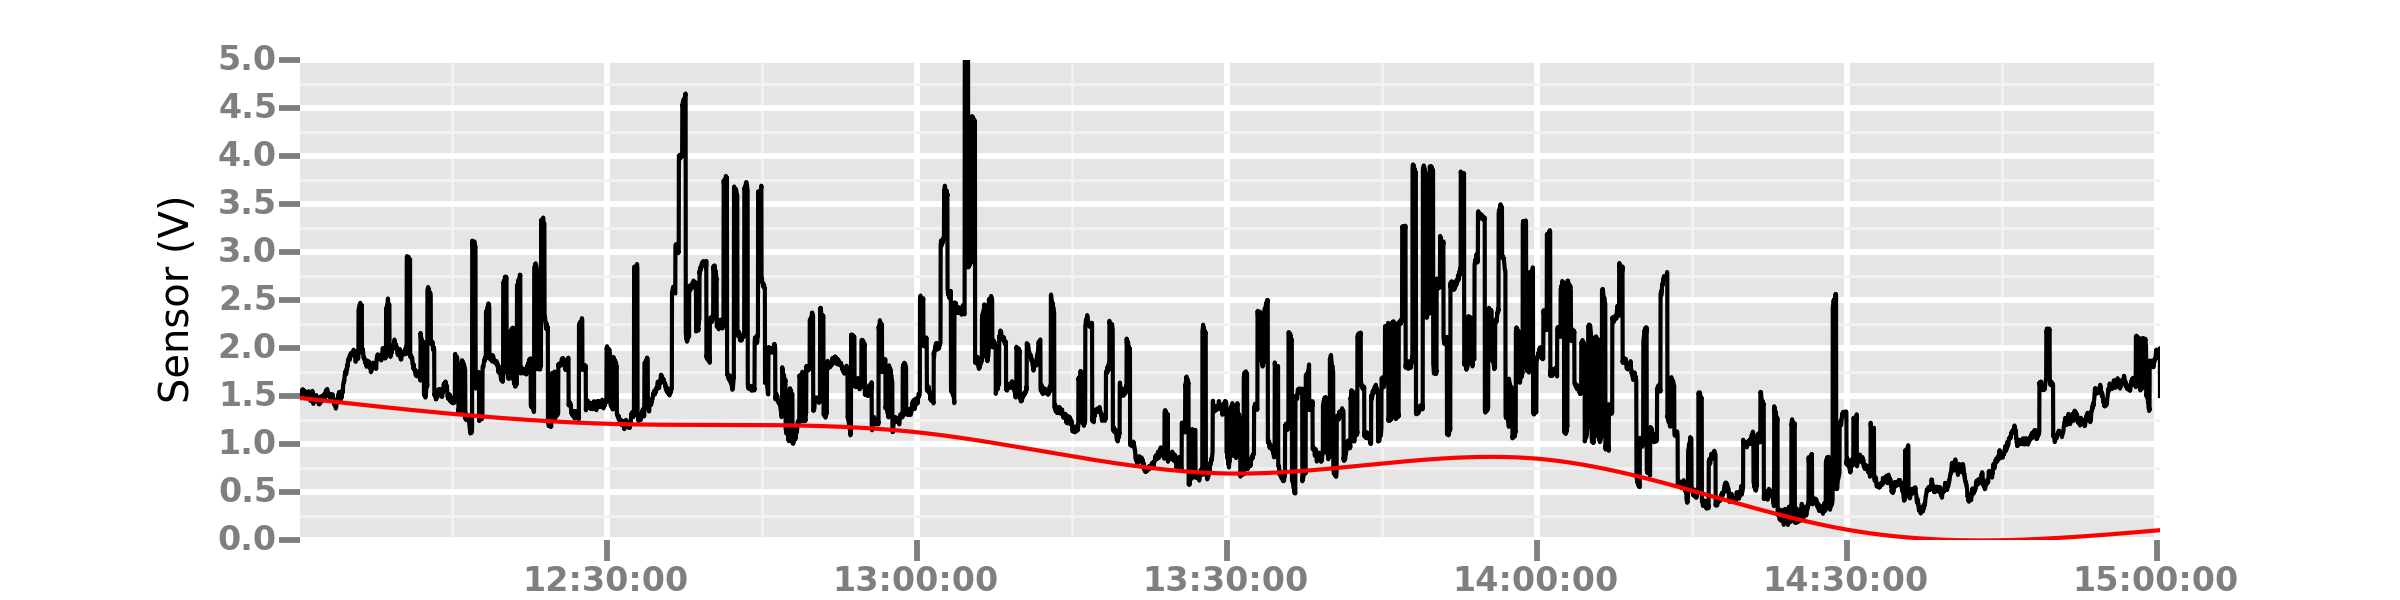
\includegraphics[width=\linewidth]{Spline_fit}
	\captionof{figure}{Example of baseline fit using Quantile Regression}
\end{center}

\subsubsection*{Butterworth Bandpass Filter} 
The measured data consists of a low frequency baseline drift component, a high-frequency noise component and the concentration signal which appears to occur at a frequency in between the drift and the noise. To separate out the concentration signal a Butterworth bandpass filter was applied using the scipy.signal toolbox with a frequency window of (0.01, 0.1) and order 2. After the filter was applied the voltage was converted into a boolean variable with 1 sec values above 0.08 set to 1. 

\begin{center}			
	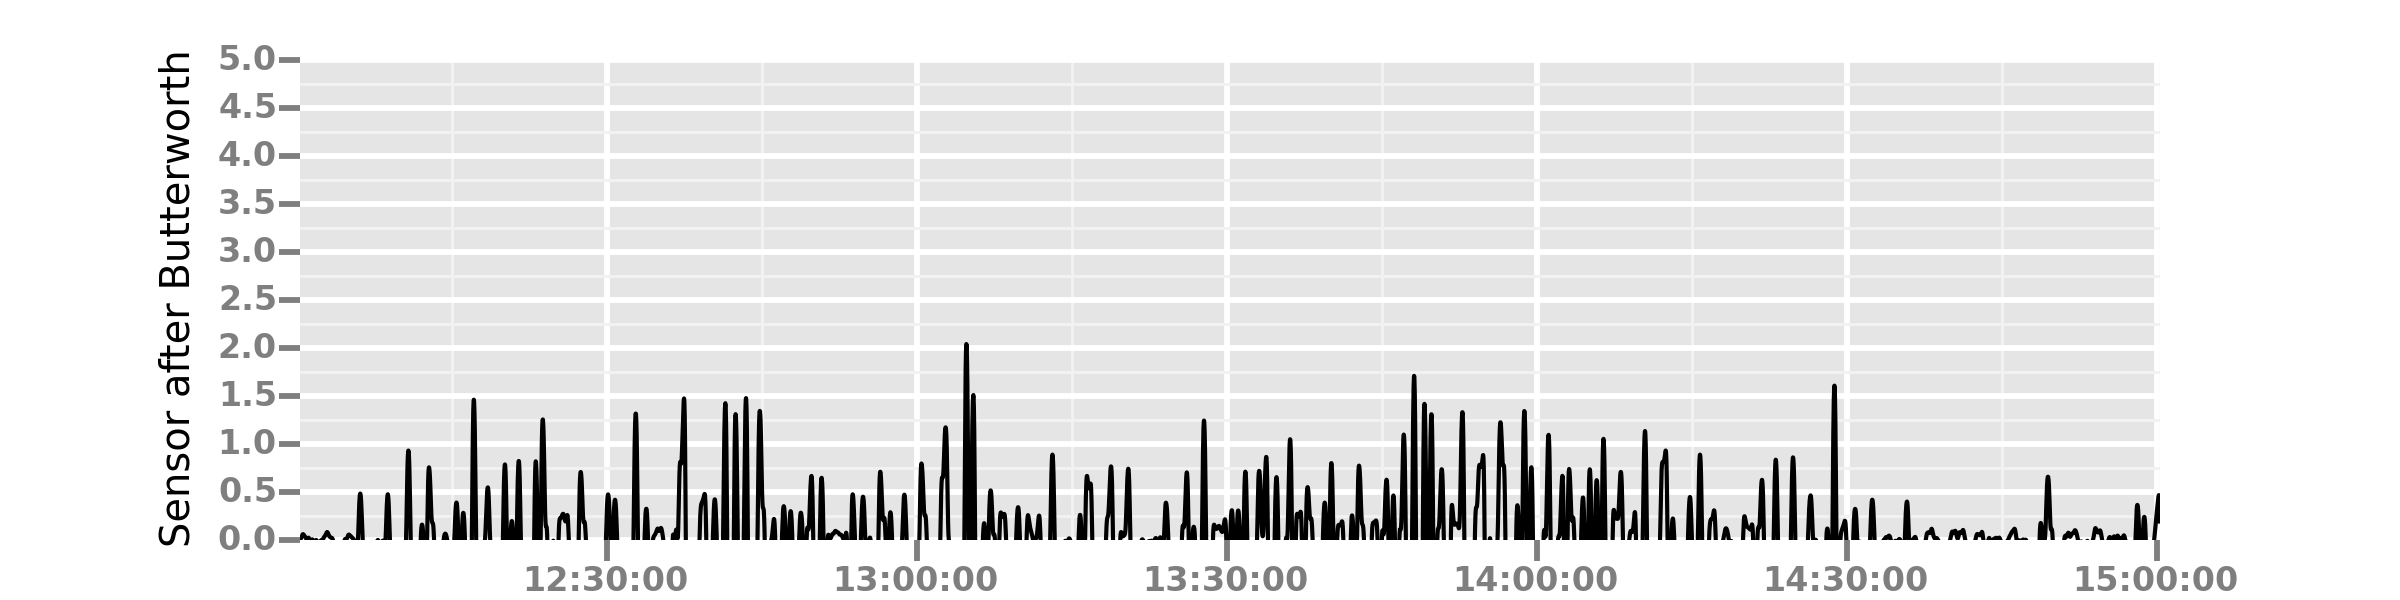
\includegraphics[width=\linewidth]{Butterworth_filt}
	\captionof{figure}{Example of sensor data after applying the bandpass filter}
\end{center}
\section*{Results}
\subsection*{Simulated Data} 
\begin{minipage}{.14\textwidth}
	\begin{itemize}			
	\item True signal was defined as boolean variable with value 1 if the 1 sec simulated signal $>$ 0.1 V, 0 otherwise.
	\item Each five minute interval was categorized into "signal present" if the mean value of the true signal was $> 0.017$, i.e. more than 5 sec of true signal in the interval. 
	\item Both the band pass filter method and the quantile regression method were able to correctly identify 80\% of the 5 min periods with true signal.
	\item The band pass filter method had false positive rate of 4 \% while the quantile regression method had a rate of 9 \%.   
	\end{itemize}
\end{minipage}
\hfill
\begin{minipage}{.14\textwidth}
	\begin{center}			
		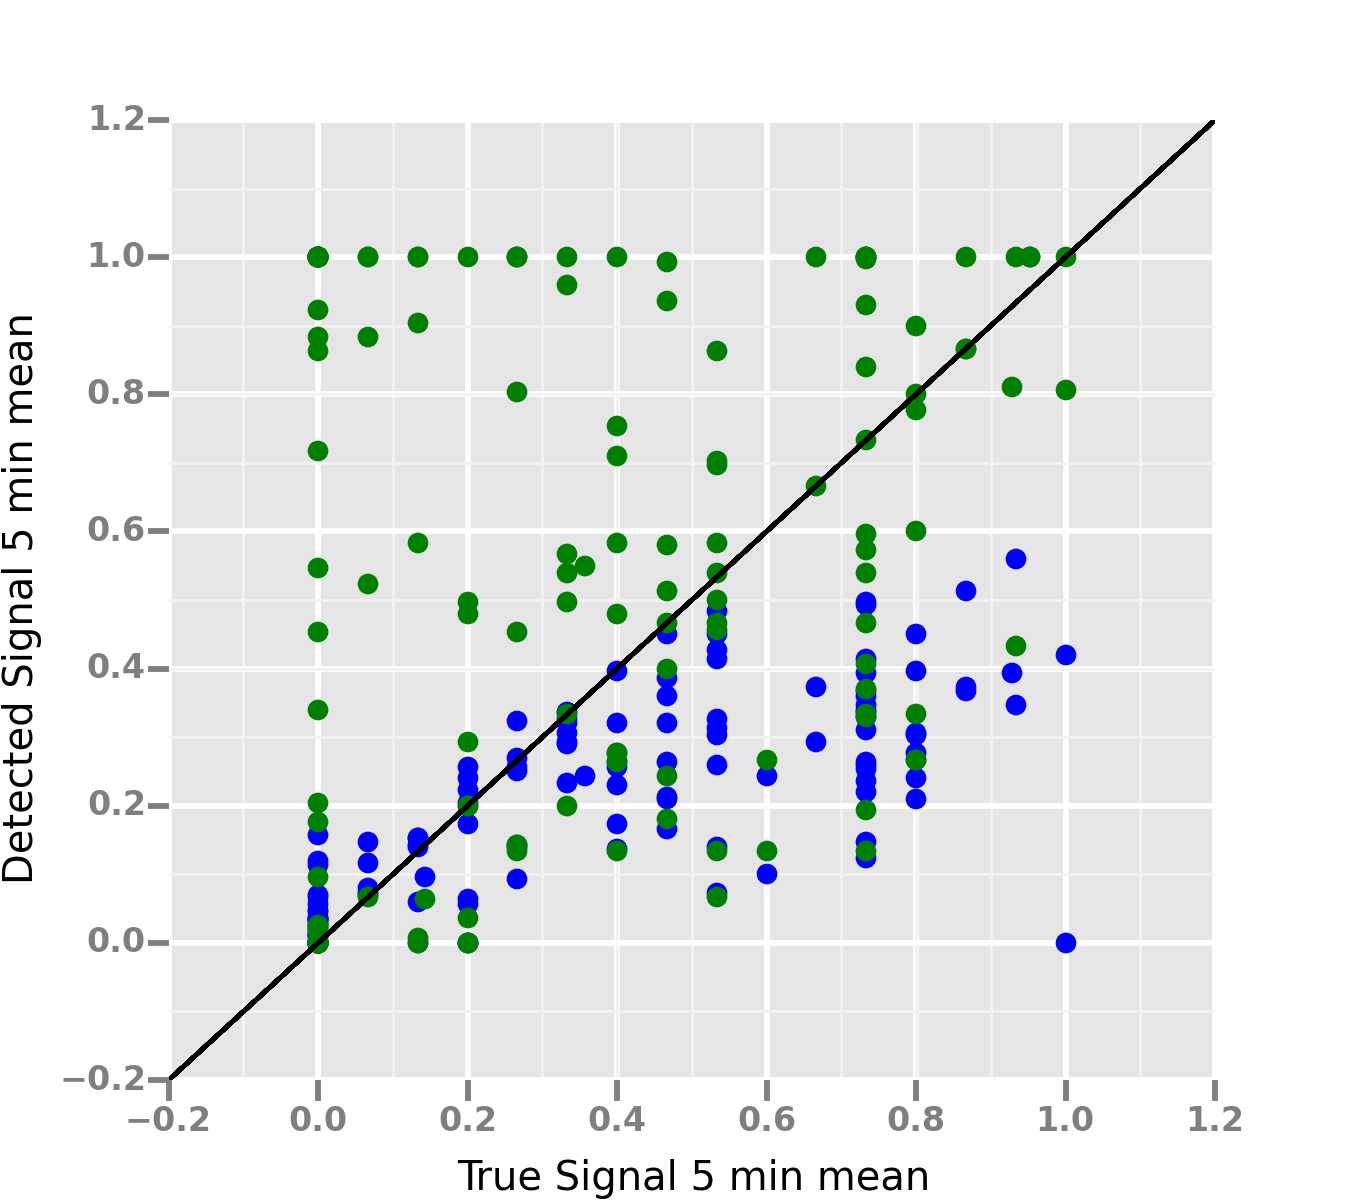
\includegraphics[width=\linewidth]{TrueVDetect}
		\captionof{figure}{True versus detected signal, green represents quantile regression and blue represents the bandpass filter.}
	\end{center}
\end{minipage}
\subsection*{Application}
\begin{itemize}
 \item The band pass filter algorithm was applied to the sensor data from 11/1/14 to 11/30/14 
 \item The resulting 5 min filtered and averaged data set was divided into (1) time periods when signal was detected at the base sensor, (2) time periods when signal was detected at the SPod sensor (3) time periods when no signal was detected.
 \item The windroses below show the distribution of 5 min wind vectors in each of the categories. The source of the emissions seems to be from a tank northeast of the sensors and is likely intermittent. 
\end{itemize} 
\begin{minipage}{.08\textwidth}
	\begin{center}			
		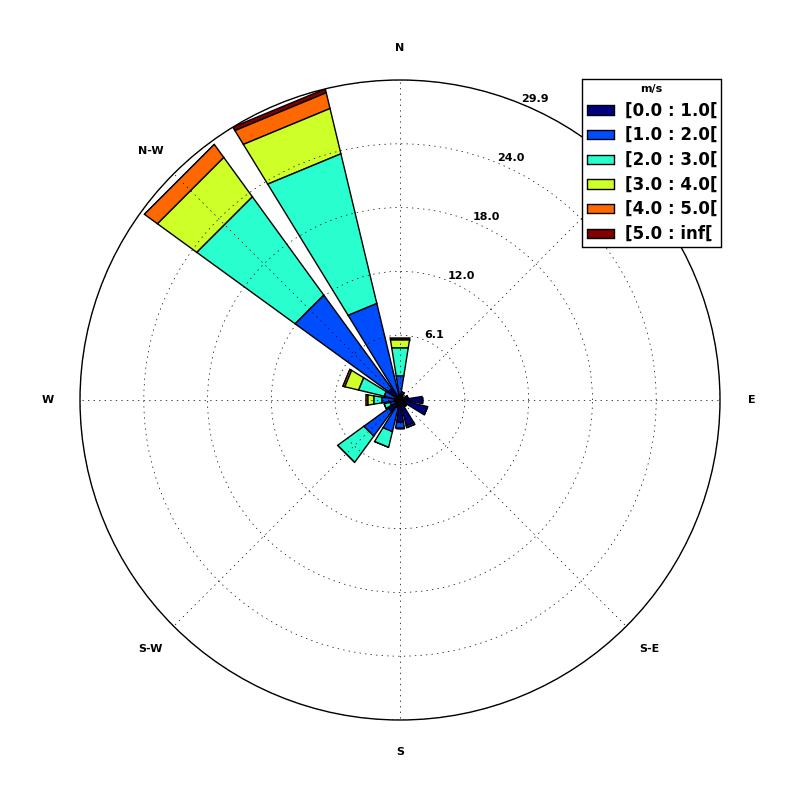
\includegraphics[width=\linewidth]{windrose_Base}
		\captionof{figure}{Signal detected at the Base sensor.}
	\end{center}
\end{minipage}
\hfill
\begin{minipage}{.08\textwidth}	
	\begin{center}			
		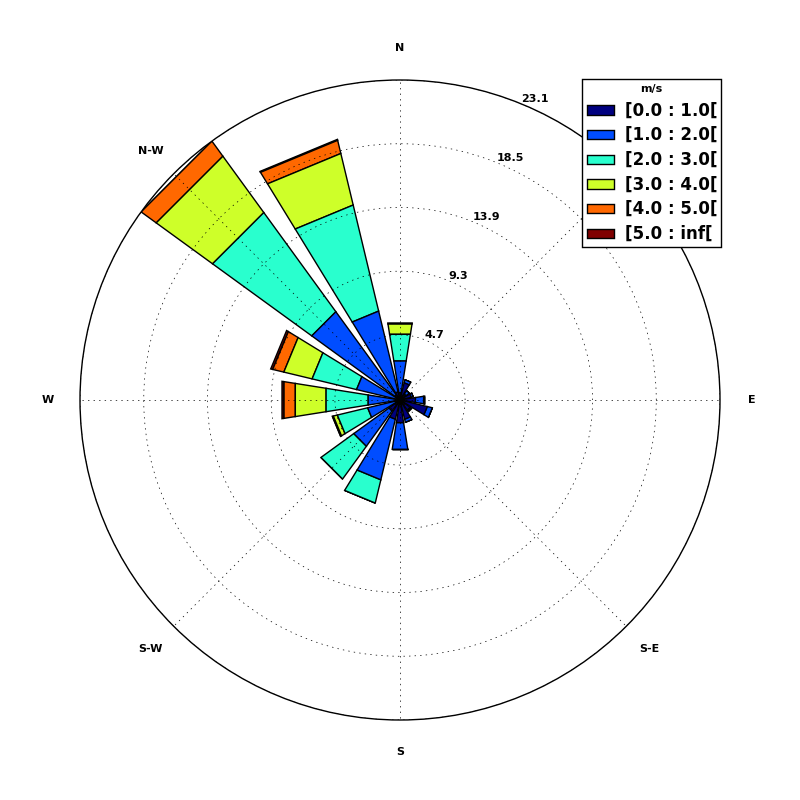
\includegraphics[width=\linewidth]{windrose_Remote}
		\captionof{figure}{Signal detected at the Remote sensor.}
	\end{center}
\end{minipage}
\hfill
\begin{minipage}{.08\textwidth}
	\begin{center}			
		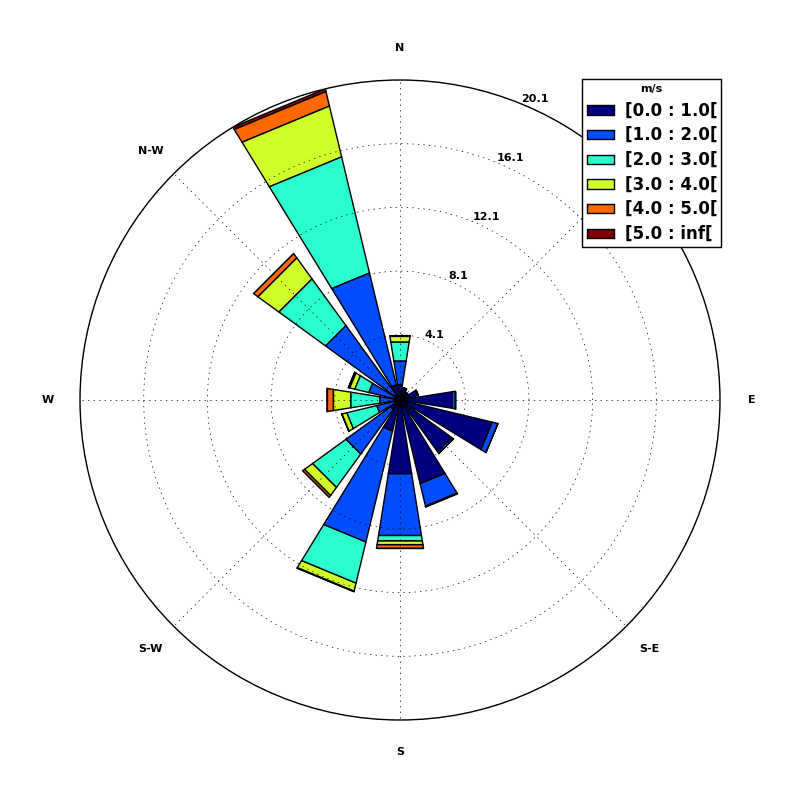
\includegraphics[width=\linewidth]{windrose_None}
		\captionof{figure}{No signal detected.}
	\end{center}
\end{minipage}

\end{multicols}

\vspace{20 pt}

\small

\printbibliography[heading=none]


\end{document}